\section{用定义证明极限的存在性}
\vspace{-14pt}
\subsection{用定义证明极限}
\vspace{-9pt}
\subsubsection{\texorpdfstring{$\epsilon-N$}方法}
\vspace{-10pt}

\begin{definition}[数列极限$\epsilon-N$语言]\label{数列极限}
    \begin{equation*}
        \forall \epsilon>0,\exists N \in \mathbb{N}^+,\mbox{使得}n>N\mbox{时,有}|x_n-A|<\epsilon\Longleftrightarrow \lim\limits_{n\to \infty} x_n=A
    \end{equation*}
\end{definition}

\begin{note}
    要证明数列极限,关键点在于根据$\epsilon$寻找对应的$N$

    (1)等价代换法:直接解$|x_n-A|<\epsilon$得$n>N(\epsilon)$,则令$N=[N(\epsilon)]+1$

    (2)放大法:若不等式$|x_n-A|<\epsilon$很难解,则可放大$|x_n-A|$为$H(n)$,使得从$H(n)<\epsilon$中可解得$n>N(\epsilon)$,

    则令$N=[N(\epsilon)]+1$

    (3)分步法:若$|x_n-A|$难以直接放大,可先假定$n$足够大,即$n>N_1$,此时$|x_n-A|$可放大为$H(n)$,使得从$H(n)<\epsilon$中可解得$n>N(\epsilon)$,令$N_2=[N(\epsilon)]+1$,再令$N=\max \{N_1,N_2\}$

    对于$\lim\limits_{x\to x_0}f(x)=a$的证明,也有类似的函数极限$\epsilon-\delta$语言
\end{note}

\begin{example}\label{例题1.2.1}
    (1)用$\epsilon-N$方法证明$\lim\limits_{n\to \infty}\sqrt[n]{n+1}=1$

    (2)设$\lim\limits_{n\to \infty} x_n=A\mbox{(有限数)}$,试证明:$\lim\limits_{n\to \infty}\frac{x_1+x_2+\cdots+x_n}{n}=A$

    (3)设$\{a_n\}$是一数列$(a_n\ne 0)$,满足$\lim\limits_{n\to \infty}a_n=0$.定义数集$P=\{ka_i\mid k\in \mathbb{Z},i\in \mathbb{N}\}$,
    试证明:对任何实数$b$,存在数列$\{b_n\}\subset P$,使得$\lim\limits b_n=b$
\end{example}

\begin{proof}
    (1)[放大法]欲解$|\sqrt[n]{n+1}-1|=\sqrt[n]{n+1}-1<\epsilon$,很难,考虑放大法.

    设$b_n=\sqrt[n]{n+1}-1$,则$n+1=(b_n+1)^n=1+C_n^1b_n+C_n^2b_n^2+\cdots $

    又$b_n>0$,故$(n+1)>C_n^2b_n=\frac{n(n-1)}{2}b_n^2$,即$b_n< \sqrt{\frac{2(n+1)}{n(n-1)}}$,

    解$\sqrt{\frac{2(n+1)}{n(n-1)}}\le\sqrt{\frac{2(n+1)+2(n-1)}{n(n-1)}}=\frac{2}{\sqrt{n-1}}<\epsilon$得$n>\frac{4}{\epsilon^2}+1$
    \begin{equation*}
        \forall \epsilon>0,\exists N=[\frac{4}{\epsilon^2}]+1 \in \mathbb{N}^+,\mbox{使得}n>N\mbox{时,有}|\sqrt[n]{n+1}-1|<\frac{2}{\sqrt{n-1}}<\epsilon\Longleftrightarrow \lim\limits_{n\to \infty}\sqrt[n]{n+1}=1
    \end{equation*}

    (2)[分步法]欲解$|\frac{x_1+x_2+\cdots+x_n}{n}-A|\le \frac{|x_1-A|+|x_2-A|+\cdots+|x_n-A|}{n}<\epsilon$

    注意到$\lim\limits_{n\to \infty} x_n=A \Longrightarrow\forall \epsilon>0,\exists N_1 \in \mathbb{N}^+,\mbox{使得}n>N_1\mbox{时,有}|x_n-A|<\frac{\epsilon}{2}$

    则$\frac{|x_1-A|+|x_2-A|+\cdots+|x_n-A|}{n}=\frac{|x_1-A|+\cdots+|x_{N_1}-A|+\cdots+|x_n-A|}{n} \le \frac{|x_1-A|+\cdots+|x_{N_1-1}|}{n}+\frac{(n-N_1)\epsilon}{n}$
    $$\le \frac{|x_1-A|+\cdots+|x_{N_1-1}|}{n}+\frac{\epsilon}{2}$$

    又$\exists N_2\in \mathbb{N}^+$,使得$n>N_2$时,有$\frac{|x_1-A|+\cdots+|x_{N_1-1}|}{n}\le \frac{\epsilon}{2}$,则
    \begin{equation*}
        \forall \epsilon>0,\exists N=\max \{N_1,N_2\},\mbox{使得}n>N\mbox{时,有}|\frac{x_1+x_2+\cdots+x_n}{n}-A|<\frac{\epsilon}{2}+\frac{\epsilon}{2}=\epsilon\Longleftrightarrow \lim\limits_{n\to \infty} \frac{x_1+x_2+\cdots+x_n}{n}=A
    \end{equation*}

    \begin{figure}[htbp!]
        \centering
        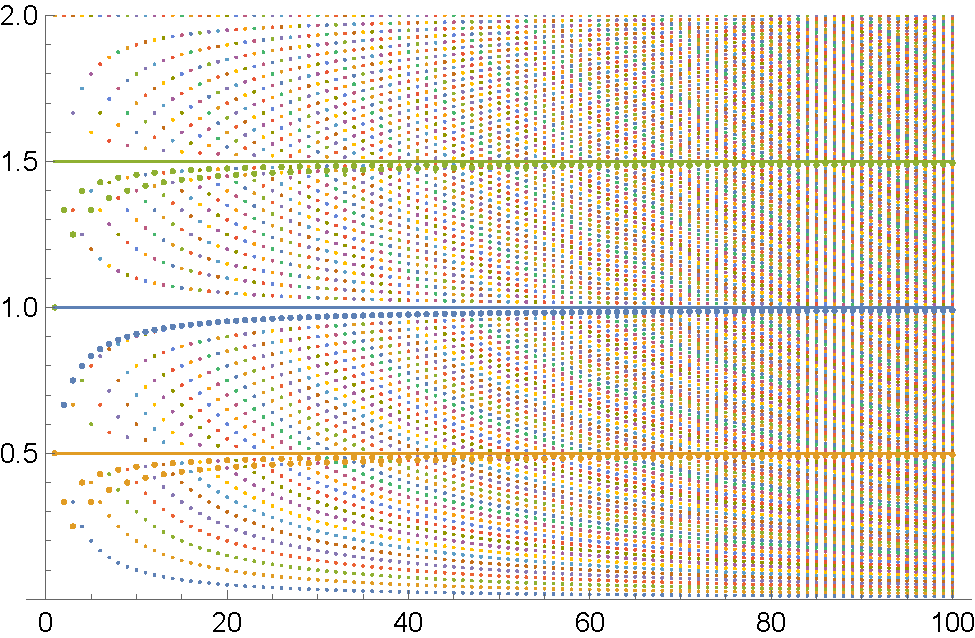
\includegraphics[width=0.5\textwidth]{../image/点列问题}
        \caption{\cref{例题1.2.1}第(3)问以$a_n=\frac{1}{n},b=0.5,1,1.5$为例}
    \end{figure}

    (3)对每个$a_i$,集合$Q_i=\{ka_i|k\in \mathbb{Z}\}$组成一个格点集:格点间距为$d_i=|a_i|$.

    对于每个实数$b$,总存在某个$k\in \mathbb{Z}$,使得$b\in[ka_i,(k+1)a_i]$,即$|b-ka_i|\le d_i$

    又$\lim\limits_{n\to \infty}a_n=0\Longrightarrow \forall \epsilon_m=\frac{1}{m}>0,\exists n_m$,有$0<|a_{n_m}|=d_{n_m}<\epsilon_m$

    对$b$和$a_{n_m}$,存在$k_m\in \mathbb{Z}$,使得$|b-k_ma_{n_m}|\le d_{n_m}<\epsilon_m$

    记$b_m=k_ma_{n_m}$,令$\epsilon_m\to 0$,即$m\to \infty$,则有$b_m\to b$,故$\{b_m\}\subset P$即为一个满足条件的数列
\end{proof}

\begin{example}
    证明:若$p_k>0(k=1,2,\cdots)$且$\lim\limits_{n\to \infty}\frac{p_n}{p_1+p_2+\cdots+p_n}=0$,$\lim\limits_{n \to \infty} a_n=a$,则$\lim\limits_{n\to \infty}\frac{p_1a_n+p_2a_{n-1}+\cdots+p_na_1}{p_1+p_2+\cdots+p_n}=a$
\end{example}

\begin{proof}

    欲解$|\frac{p_1a_n+p_2a_{n-1}+\cdots+p_na_1}{p_1+p_2+\cdots+p_n}-a|\le \frac{p_1|a_n-a|+\cdots+p_n|a_1-a|}{p_1+p_2+\cdots+p_n}<\epsilon$

    注意到$\lim\limits_{n\to \infty} a_n=a \Longrightarrow\forall \epsilon>0,\exists N_1 \in \mathbb{N}^+,\mbox{使得}n>N_1\mbox{时,有}|a_n-a|<\frac{\epsilon}{2}$,则
    $$\frac{p_1|a_n-a|+\cdots+p_{n-N_1}|a_{N_1+1}-a|+\cdots+p_n|a_1-a|}{p_1+p_2+\cdots+p_n}< \frac{\epsilon}{2}\cdot \frac{p_1+\cdots+p_{n-N_1}}{p_1+p_2+\cdots+p_n}+\frac{p_{n-N_1+1}|a_{N_1}-a|+\cdots+p_n|a_1-a|}{p_1+p_2+\cdots+p_n}$$
    $$<\frac{\epsilon}{2}+\frac{p_{n-N_1+1}|a_{N_1}-a|+\cdots+p_n|a_1-a|}{p_1+p_2+\cdots+p_n}$$

    设$M=\max \{|a_{N_1}-a|,\cdots,|a_1-a|\}$,
    则$\frac{p_{n-N_1+1}|a_{N_1}-a|+\cdots+p_n|a_1-a|}{p_1+p_2+\cdots+p_n}<\frac{p_{n-N_1+1}+\cdots+p_n}{p_1+p_2+\cdots+p_n}M$
    \begin{equation*}
        0<\frac{p_{n-i+1}}{p_1+p_2+\cdots+p_n}<\frac{p_{n-i+1}}{p_1+p_2+\cdots+p_{n-i+1}}\to 0\Longrightarrow \lim\limits_{n\to \infty}\frac{p_{n-i+1}}{p_1+p_2+\cdots+p_n}=0\quad i=2,\cdots,N_1
    \end{equation*}

    故$\lim\limits_{n\to \infty} \frac{p_{n-N_1+1}+\cdots+p_n}{p_1+p_2+\cdots+p_n} = 0
        \Longrightarrow
        \exists N_2\in \mathbb{N}^+$,使得$n>N_2$时,$\frac{p_{n-N_1+1}+\cdots+p_n}{p_1+p_2+\cdots+p_n}<\frac{\epsilon}{2M}$
    $$\forall \epsilon,\exists N=\max \{N_1,N_2\},\mbox{使得}n>N\mbox{时,有}|\frac{p_1a_n+p_2a_{n-1}+\cdots+p_na_1}{p_1+p_2+\cdots+p_n}-a|<\frac{\epsilon}{2}+\frac{\epsilon}{2M}\cdot M=\epsilon$$
    $$\Longrightarrow \lim\limits_{n\to \infty}\frac{p_1a_n+p_2a_{n-1}+\cdots+p_na_1}{p_1+p_2+\cdots+p_n}=a$$
\end{proof}

\begin{example}
    设实数列$\{x_n\}$满足$\lim\limits_{n\to \infty}(x_n-x_{n-2})=0$,证明:$\lim\limits_{n\to \infty}\frac{x_n-x_{n-1}}{n}=0$
\end{example}

\begin{proof}

    欲解$|\frac{x_n-x_{n-1}}{n}|<\epsilon$.

    设$y_n=|x_n-x_{n-1}|$,则$|x_n-x_{n-2}|=|x_n-x_{n-1}+x_{n-1}-x_{n-2}|\ge ||x_n-x_{n-1}|+|x_{n-1}-x_{n-2}||=|y_n-y_{n-1}|\ge 0$

    故$\lim\limits_{n\to \infty}|y_n-y_{n-1}|=0
        \Longrightarrow \forall \epsilon>0,\exists N_1\in \mathbb{N}^+,\mbox{使得}n>N_1\mbox{时},|y_n-y_{n-1}|<\epsilon$

    则$$|\frac{x_n-x_{n-1}}{n}|=\frac{y_n}{n}\le
        \frac{|y_n-y_{n-1}|+|y_{n-1}-y_{n-2}|+\cdots +|y_{N_1+1}-y_{N_1}|}{n}+\frac{y_{N_1}}{n}<\frac{(n-N_1)}{n}\cdot \frac{\epsilon}{2}+\frac{y_{N_1}}{n}<\frac{\epsilon}{2}+\frac{y_{N_1}}{n}$$

    又$\exists N_2\in \mathbb{N}^+$,使得$n>N_2$时,有$\frac{y_{N_1}}{n}<\frac{\epsilon}{2}$

    故$\forall \epsilon,\exists N=\max \{N_1,N_2\}$,使得$n>N$时,有$|\frac{x_n-x_{n-1}}{n}|<\frac{\epsilon}{2}+\frac{\epsilon}{2}=\epsilon\Longrightarrow \lim\limits_{n\to \infty}\frac{x_n-x_{n-1}}{n}=0$
\end{proof}

\begin{definition}[函数极限$\epsilon-\delta$语言]
    \begin{equation*}
        \forall \epsilon>0,\exists \delta>0,\mbox{使得}0<|x-x_0|<\delta\mbox{时,有}|f(x)-a|<\epsilon\Longleftrightarrow \lim\limits_{x\to x_0} f(x)=a
    \end{equation*}
\end{definition}

\begin{example}
    按极限定义($\epsilon-\delta$语言)证明:$\lim\limits_{x\to 1}\sqrt{\frac{7}{16x^2-9}}=1$
\end{example}

\begin{proof}
    欲解$|\sqrt{\frac{7}{16x^2-9}}-1|<\epsilon$得$|x-1|<\delta(\epsilon)$.考虑放缩.
    $$|\sqrt{\frac{7}{16x^2-9}}-1|=|\frac{\frac{7}{16x^2-9}-1}{\sqrt{\frac{7}{16x^2-9}}+1}|\le |\frac{7}{16x^2-9}-1|=\frac{16|x+1||x-1|}{|(4x+3)(4x-3)|}\le \frac{16|x+1||x-1|}{3|4x-3|}$$

    还是较难. 考虑分步法,设$|x-1|<1$,则$0<x<2\Longrightarrow |x+1|<3\Longrightarrow \frac{16|x+1||x-1|}{3|4x-3|}<\frac{16|x-1|}{|4x-3|}=\frac{4|x-1|}{|x-\frac{3}{4}|}$

    进一步,设$|x-1|<\frac{1}{8}$,则$\frac{7}{8}<x<\frac{9}{8}\Longrightarrow |x-\frac{3}{4}|>\frac{1}{8}\Longrightarrow \frac{16|x+1||x-1|}{3|4x-3|}<32|x-1|$
    $$\forall \epsilon>0,\exists \delta=\min \{\frac{1}{8},\frac{1}{32}\epsilon\},\mbox{使得}0<|x-1|<\delta\mbox{时,有}|\sqrt{\frac{7}{16x^2-9}}-1|<\epsilon\Longrightarrow \lim\limits_{x\to 1}\sqrt{\frac{7}{16x^2-9}}=1$$
\end{proof}

\subsubsection{拟合法}

\begin{note}
    为了证明$\lim \limits_{n \to \infty}x_n=A$,关键在于证明$|x_n-A|$能够任意小. 为此,一般尽可能将$x_n$化简.值得注意的是,有时候$x_n$难以化简,反而$A$能够“化繁”,写成与$x_n$类似的形式.这种方法称为“拟合法”.“拟合法”思想的实质,是将单位“1”进行适当的分解.
\end{note}

\vspace{8pt}
\begin{example}\label{例题1.2.5}
    设$x\to 0$时,$f(x)\thicksim x,x_n=\sum\limits_{i=1}^{n}f(\frac{2i-1}{n^2}a)$,试证明$\lim \limits_{n \to \infty}x_n=a(a>0)$
\end{example}

\begin{proof}
    注意到$a=\sum\limits_{i=1}^{n}\frac{2i-1}{n^2}a$,从而有$
        |x_n-a|
        =|\sum\limits_{i=1}^{n}f(\frac{2i-1}{n^2}a)-\sum\limits_{i=1}^{n}\frac{2i-1}{n^2}a|
        =\sum\limits_{i=1}^{n}|f(\frac{2i-1}{n^2}a)-\frac{2i-1}{n^2}a|$

    若能证明$\forall \epsilon>0$时,
    \begin{equation}\label{式1.2.1}
        \exists N\in \mathbb{N}^+,\mbox{使得}n>N\mbox{时},|f(\frac{2i-1}{n^2}a)-\frac{2i-1}{n^2}a|<\frac{2i-1}{n^2}\epsilon\quad i=1,2,\cdots,n
    \end{equation},

    则有$n>N$时,
    $|x_n-a|
        =\sum\limits_{i=1}^{n}|f(\frac{2i-1}{n^2}a)-\frac{2i-1}{n^2}a|
        <\sum\limits_{i=1}^{n}\frac{2i-1}{n^2} \epsilon=\epsilon
    $,即$\lim \limits_{n \to \infty}x_n=a(a>0)$得证

    欲证\cref{式1.2.1},即证$$\exists N\in \mathbb{N}^+,\mbox{使得}n>N\mbox{时},|\frac{f(\frac{2i-1}{n^2}a)}{\frac{2i-1}{n^2}a}-1|<\frac{\epsilon}{a}\quad i=1,2,\cdots,n$$

    事实上,由于$x\to 0\mbox{时},f(x)\thicksim x \Longrightarrow \forall \epsilon,\exists \delta>0,0<|x|<\delta$时,$|\frac{f(x)}{x}-1|<\frac{\epsilon}{a}$

    令$\frac{2i-1}{n^2}a
        <\frac{2n-1}{n^2}a
        <\frac{2n}{n^2}a
        =\frac{2}{n^2}a<\frac{2a}{n}
        <\delta$
    解得$n>\frac{2a}{\delta}$,令$N=[\frac{2a}{\delta}]+1$,

    则$n>N\mbox{时},0<\frac{2i-1}{n^2}a<\delta\Longrightarrow|\frac{f(\frac{2i-1}{n^2}a)}{\frac{2i-1}{n^2}a}-1|<\frac{\epsilon}{a}$.得证
\end{proof}

\begin{practice}
    证明:

    (1)$\lim \limits_{n \to \infty} \prod \limits_{i=1}^{n} (1+\frac{2i-1}{n^2}a^2)=e^{a^2}$\quad
    (2)$\lim \limits_{n \to \infty}  \prod \limits_{i=1}^{n+1} \cos \frac{\sqrt{2i-1}}{n}a^2=e^{-\frac{a^4}{2}}$
\end{practice}

\begin{proof}
    (1)两边取对数,得需证
    $\lim \limits_{n \to \infty} \sum \limits_{i=1}^{n} \ln(1+\frac{2i-1}{n^2}a^2)=a^2$

    $x\to 0$时,$f(x)=\ln (1+x) \thicksim x $,则由\cref{例题1.2.5}得,$\lim \limits_{n \to \infty} \sum \limits_{i=1}^{n} \ln(1+\frac{2i-1}{n^2}a^2)
        =\lim \limits_{n \to \infty} \sum \limits_{i=1}^{n} f(\frac{2i-1}{n^2}a^2)
        =a^2$

    (2)两边取对数,得需证
    $\lim \limits_{n \to \infty} \sum \limits_{i=1}^{n+1} \ln(\cos \frac{\sqrt{2i-1}}{n}a^2)=-\frac{a^4}{2}$

    $x\to 0$时,$f(x)=\ln \cos x=\ln [1+(\cos x-1)] \thicksim (\cos x-1) \thicksim -2\sin^2 \frac{x}{2} \thicksim -\frac{x^2}{2}$

    同\cref{例题1.2.5}考虑拟合法,可证$\lim \limits_{n \to \infty} \sum \limits_{i=1}^{n} \ln(1+\frac{2i-1}{n^2}a^2)
        =\lim \limits_{n \to \infty} \sum \limits_{i=1}^{n} f(\frac{\sqrt{2i-1}}{n}a^2)
        =-\frac{(a^2)^2}{2}
        =-\frac{a^4}{2}$
\end{proof}

\begin{practice}\label{小试牛刀1.2.2}
    设$\lim \limits_{n \to \infty} a_n = a$,试证:
    \begin{equation*}
        \lim \limits_{n \to \infty} \frac{1}{2^n} (a_0+C_n^1 a_1 + C_n^2 a_2 + \cdots + C_n^k a_k + \cdots + a_n)=a
    \end{equation*}
\end{practice}

\begin{proof}
    $a = \frac{2^n}{2^n} a
        =\frac{\sum\limits_{k=0}^{n} C_n^k}{2^n} a
        =\frac{1}{2^n} \sum\limits_{k=0}^{n} C_n^k a \Longrightarrow |\frac{1}{2^n} \sum\limits_{k=0}^{n} C_n^k a_k - a|
        =|\frac{1}{2^n} \sum\limits_{k=0}^{n} C_n^k a_k - \frac{1}{2^n} \sum\limits_{k=0}^{n} C_n^k a|
        \le \frac{1}{2^n} \sum\limits_{i=0}^{n} C_n^k |a_k-a|$

    又$\lim \limits_{n \to \infty} a_n = a
        \Longrightarrow \forall \epsilon>0,\exists k_0 \in \mathbb{N}^+,\mbox{使得}k>k_0时,|a_k-a|<\frac{\epsilon}{2}$

    而$k<k_0$时,记$M=\max |a_k-a|$,则$|a_k-a|\le M$

    故$\frac{1}{2^n} \sum\limits_{k=0}^{n} C_n^k |a_k-a|=\frac{1}{2^n} \sum\limits_{k=0}^{k_0-1} C_n^k |a_k-a| + \frac{1}{2^n} \sum\limits_{k=k_0}^{n} C_n^k |a_k-a|< \frac{Mk_0n^{k_0}}{2^n} + \frac{\epsilon}{2}$

    又$\lim \limits_{n \to \infty} \frac{Mk_0n^{k_0}}{2^n}=0 \Longrightarrow \exists N>k_0>0$,使得$n>N$时,有$|\frac{1}{2^n} \sum\limits_{k=0}^{n} C_n^k a_k - a| < \frac{Mk_0n^{k_0}}{2^n} + \frac{\epsilon}{2}<\frac{\epsilon}{2} + \frac{\epsilon}{2}<\epsilon$

    即$\lim \limits_{n \to \infty} \frac{1}{2^n} (a_0+C_n^1 a_1 + C_n^2 a_2 + \cdots + C_n^k a_k + \cdots + a_n)=a$得证
\end{proof}

\begin{practice}
    若\cref{小试牛刀1.2.2}中$\frac{C_n^k}{2^n}$改为一般的实数$\alpha_{n,k},\forall n\in \mathbb{N}:k=0,1,\cdots,n$,问$a_{n,k}$应该满足什么条件,该命题依然成立?即当$\lim \limits_{n \to \infty}a_n=a\Longrightarrow \lim \limits_{n \to \infty} \sum\limits_{k=0}^{n} \alpha_{n,k}a_k=a$
\end{practice}

\begin{solution}
    $\sum\limits_{k=1}^{n} a_{n,k}=1$
\end{solution}

\subsubsection{用邻域描述极限}
\begin{definition}[邻域]
    区间$(a-\epsilon,a+\epsilon)$称为点$a$的$\epsilon-$领域,用$U(a,\epsilon)$表示。

    区间$(a-\epsilon,a)\bigcup (a,a+\epsilon)$称为$a$的$\epsilon-$去心邻域,用$\overset{\circ}{U}(a,\epsilon)$表示。
\end{definition}

\begin{note}
    
    使用邻域语言,可以将定义\ref{数列极限}中的$\epsilon-\delta$语言表述为以下的等价形式

    \begin{enumerate}
        \item $\lim \limits_{n \to \infty} a_n = a \Longleftrightarrow \forall \epsilon>0, \exists N\in \mathbb{N}^+,\mbox{使得}\forall n>N\mbox{时},\mbox{有} a_n\in U(a,\epsilon)$
        \item $\lim \limits_{n \to \infty} a_n = a \Longleftrightarrow \forall \epsilon>0, \mbox{只有有限个}n\in \mathbb{N^+},\mbox{使得}a_n\notin U(a,\epsilon)$
        \item $\lim \limits_{n \to \infty} a_n = a \Longleftrightarrow \forall \epsilon>0,U(a,\epsilon)$之外仅有$a_n$的有限项
    \end{enumerate}
\end{note}

\vspace{3pt}
\begin{example}
    设$f:\mathbb{N} \rightarrow \mathbb{N}_1$,$n=f(m)$($\mathbb{N}$和$\mathbb{N}_1$都是全体自然数组成的空间),且$\forall n\in \mathbb{N}:f^{-1}(n)$为有限集.试证明:若$\lim \limits_{n \to \infty} a_n =a$,则$\lim \limits_{m \to \infty} a_{f_{(m)}}=a$
\end{example}

\begin{proof}

    [法1]$\lim \limits_{n \to \infty} a_n = a \Longleftrightarrow \forall \epsilon>0,U(a,\epsilon)$之外仅有$a_n$的有限项

    把这$U(a,\epsilon)$之外的有限项记作$\{a_{n_j}\}_{j=1}^k={a_{}}=\{a_{n_1},a_{n_2},\cdots,a_{n_k}\}$

    又根据题意得,$f^{-1}(n_j)=\{m|n_j=f_m\}$为有限集,它们的并$E=\underset{j=1}{\overset{k}{\bigcup}} \{m|n_j=f(m)\}$仍然是有限集。

    故$\forall \epsilon>0,U(a,\epsilon)$之外仅有$a_{f_{(m)}}$的有限项:$\{a_{f_{(m)}|m\in E}\} \Longleftrightarrow \lim \limits_{m \to \infty} a_{f_{(m)}}=a$

    [法2]$\lim \limits_{n \to \infty} a_n = a \Longleftrightarrow \forall \epsilon>0, \exists N\in \mathbb{N}^+,\mbox{使得}\forall n>N\mbox{时},\mbox{有} a_n\in U(a,\epsilon)$

    又根据题意得,$\forall n\in \mathbb{N}:f^{-1}(n)$为有限集,则$\underset{n\le N}{\bigcup} f^{-1}(n)$为有限集,$\exists M=\max \underset{n\le N}{\bigcup} f^{-1}(n)$,

    则$m>M$时,有$a_m\in U(a,\epsilon) \Longrightarrow \lim \limits_{m \to \infty} a_{f_{(m)}}=a$

    [法3]只需证明$\{f(m)\}_{m=1}^{\infty}$是$\{n\}_{n=1}^{\infty}$的子列(不需要单调增,只需要趋于$+\infty$即可),则根据数列与子列关系,
    
    有$\lim \limits_{n \to \infty} a_n=a \Longrightarrow \lim \limits_{m \to \infty} a_{f_{(m)}}=a$

    事实上,若$\{f(m)\}_{m=1}^{\infty}$是$\{n\}_{n=1}^{\infty}$的子列,则说明$\{f(m)\}_{m=1}^{\infty}$只是$\{n\}_{n=1}^{\infty}$中的有限项,也就是说:$\{n\}_{n=1}^{\infty}$中的有限项对应着$\{f(m)\}_{m=1}^{\infty}$中的无穷多项。

    因此,至少存在一个$n$通过$n=f(m)$对应着无穷多个$m$。这与题设“$\forall n\in \mathbb{N}:f^{-1}(n)$为有限集”矛盾
\end{proof}

\subsection{用柯西收敛准则证明极限}
\begin{theorem}[柯西(Cauchy)收敛准则]
    数列$\{x_n\}$收敛 
    
    $\Longleftrightarrow \forall \epsilon>0,\exists N\in \mathbb{N}^+$,使得$\forall m,n>N$,有$|x_m-x_n|<\epsilon$

    $\Longleftrightarrow \forall \epsilon>0,\exists N\in \mathbb{N}^+$,使得$n>N\mbox{时},\forall p\in \mathbb{N}^+$,有$|x_{n+p}-x_n|<\epsilon$
\end{theorem}

\begin{example}
    设$\displaystyle x_n=\frac{\sin 1}{2}+\frac{\sin 2}{2^2}+\cdots+\frac{\sin n}{2^n}$,试证$\{x_n\}$收敛
\end{example}

\begin{proof}
    $$|x_{n+p}-x_n|
    =|\frac{\sin (n+1)}{2^{n+1}}+\cdots+\frac{\sin (n+p)}{2^{n+p}}|
    \le |\frac{\sin (n+1)}{2^{n+1}}|+\cdots+|\frac{\sin (n+p)}{2^{n+p}}|
    \le \frac{1}{2^{n+1}}+\cdots+\frac{1}{2^{n+p}}$$
    $$=\frac{1}{2^{n+1}} \cdot \frac{1-\frac{1}{2^p}}{1-\frac{1}{2}}
    <\frac{1}{2^n}<\frac{1}{n}$$

    解$|x_{n+p}-x_n|<\frac{1}{n}<\epsilon$得$n>\frac{1}{\epsilon}$

    因此,$\forall \epsilon>0,\exists N=[\frac{1}{\epsilon}]+1\in \mathbb{N}^+$,使得$n>N$时,$\forall p\in \mathbb{N}^+$,有$|x_{n+p}-x_n|<\epsilon$

    由柯西收敛准则得,数列$\{x_n\}$收敛 
\end{proof}

\clearpage
\begin{example}
    判断以下命题的真伪:

    数列$\{a_n\}$存在极限$\lim \limits_{n \to \infty} a_n =a$的充分必要条件是:对任意$p\in \mathbb{N}^+$,都有$\lim \limits_{n \to \infty}|a_{n+p}-a_n|=0$
\end{example}

\begin{solution}
    
    该命题不对.如$a_n=\sqrt{n}$,虽然$\lim \limits_{n \to \infty}|a_{n+p}-a_n|
    =\lim \limits_{n \to \infty}|\sqrt{n+p}-\sqrt{n}|
    =\lim \limits_{n \to \infty} \frac{p}{\sqrt{n+p}+\sqrt{n}}
    =0$

    但$\lim \limits_{n \to \infty} a_n =+\infty$,即数列$\{a_n\}$不存在极限
\end{solution}

\subsection{否定形式及 \texorpdfstring{$\forall$}{} 和 \texorpdfstring{$\exists$}{} 的使用法则}

\begin{theorem}[数列发散]
    数列$\{x_n\}$发散

    $\Longleftrightarrow \forall A \in \mathbb{R}, \exists \epsilon_0 > 0,\forall N\in \mathbb{N}^+,\exists n_0 > N$,使得$|x_{n_0}-A|\ge \epsilon_0$ \qquad (极限定义的否定形式)
    
    $\Longleftrightarrow \exists \epsilon_0 > 0,\forall N\in \mathbb{N}^+,\exists m_0,n_0 > N$,使得$|x_{m_0}-x_{n_0}|\ge \epsilon_0 $ \qquad (柯西收敛准则的否定形式1)

    $\Longleftrightarrow \exists \epsilon_0 > 0,\forall N\in \mathbb{N}^+,\exists n_0>N,p_0\in \mathbb{N}^+$,使得$|x_{n_0+p_0}-x_{n_0}|\ge \epsilon_0 $\qquad (柯西收敛准则的否定形式2)
\end{theorem}

\begin{note}若能证明以下结论,也能说明数列$\{x_n\}$发散:
    \begin{enumerate}
        \item $\forall A\in \mathbb{R},\mbox{当} n\to \infty \mbox{时,有}|a_n-A| \ge \varphi (n) \to a \ne 0$
        \item $\forall n\in \mathbb{N}^+,、\mbox{当}p\to \infty \mbox{时,有} |x_{n+p}-x_n| \ge \varphi(n,p) \to a \ne 0$
    \end{enumerate}
\end{note}

\begin{example}
    证明:$\lim \limits_{n \to \infty} \sin n$不存在
\end{example}

\begin{proof}
    
    [法1]根据极限定义的否定形式,我们需证明:$ \forall A \in \mathbb{R}, \exists \epsilon_0 > 0,\forall N\in \mathbb{N}^+,\exists n_0 > N$,使得$|x_{n_0}-A|\ge \epsilon_0$

    当$|A|>1$时,$\forall n\in \mathbb{N}^+,|\sin n - A| \ge ||\sin n|-|A||=|A|-|\sin n|\ge |A|-1>0$

    当$0\le A \le 1$时,$\forall N\in \mathbb{N}^+,\exists n_0=[(2N\pi - \frac{\pi}{2})+\frac{\pi}{4}]>N$,
    
    有$2N\pi - \frac{\pi}{2}-\frac{\pi}{4} < n_0 < 2N\pi -\frac{\pi}{2}+\frac{\pi}{4} \Longrightarrow -1 < \sin n_0 < -\frac{\sqrt{2}}{2}$,
    则$|\sin n_0 -A|=A-\sin n_0 > A+\frac{\sqrt{2}}{2}\ge \frac{\sqrt{2}}{2}$

    当$-1\le A<0$时,$\forall N\in \mathbb{N}^+,\exists n_0=[(2N\pi + \frac{\pi}{2})+\frac{\pi}{4}]>N$,
    
    有$2N\pi + \frac{\pi}{2}-\frac{\pi}{4} < n_0 < 2N\pi +\frac{\pi}{2}+\frac{\pi}{4} \Longrightarrow \frac{\sqrt{2}}{2} < \sin n_0 < 1 $,
    则$|\sin n_0 -A|=\sin n_0 - A > \frac{\sqrt{2}}{2} - A \ge \frac{\sqrt{2}}{2}$

    [法2]根据柯西收敛准则的否定形式1,我们需证明$\exists \epsilon_0 > 0,\forall N\in \mathbb{N}^+,\exists m_0,n_0 > N$,使得$|x_{m_0}-x_{n_0}|\ge \epsilon_0 $

    事实上,取$\epsilon_0=\frac{\sqrt{2}}{2},m_0=[2N\pi + 2\pi] ,n_0=[2N\pi + \frac{3\pi}{4}]$

    有$m_0,n_0>N$,且$2N\pi + \pi <m_0< 2N\pi + 2\pi,2N\pi +\frac{\pi}{4}<n_0<2N\pi + \frac{3\pi}{4}\Longrightarrow -1<\sin m_0<0,\frac{\sqrt{2}}{2}<\sin n_0<1$,
    
    则$|\sin m_0-\sin n_0|=\sin n_0-\sin m_0>\frac{\sqrt{2}}{2}=\epsilon_0$

    [法3]用反证法。假设$\lim \limits_{n \to \infty} \sin n=A$.
    
    由$\sin(n+2)-\sin n=\sin(n+1+1)-\sin (n+1-1)=2sin 1 \cos (n+1)$得
    
    $\lim \limits_{n \to \infty} \cos (n+1)=\lim \limits_{n \to \infty} [\sin(n+2)-\sin n]=A-A=0$,即$\lim \limits_{n \to \infty} \cos n = 0$

    则$A=\lim \limits_{n \to \infty} \sin n = \lim \limits_{n \to \infty} \sqrt{1-\cos^2 n} = 1$

    又$A=\lim \limits_{n \to \infty} \sin 2n=\lim \limits_{n \to \infty} 2\cos n \sin n = 0$

    所以产生矛盾。$\lim \limits_{n \to \infty} \sin n$不存在
\end{proof}



\begin{example}\label{例题1.2.10}
    证明:数列$S_n=\sum\limits_{k=1}^{n} \frac{1}{k}(n=1,2,\cdots)$发散
\end{example}

\begin{proof}
    
    $\forall n\in \mathbb{N}^+,|S_{n+p}-S_n|=\frac{1}{n+1}+\cdots+\frac{1}{n+p}\ge \frac{p}{n+p} \to 1 \ne 0(p \to \infty)$

    故可取$\epsilon_0=\frac{1}{2}$,则由极限的保号性得$\forall N\in \mathbb{N}^+,\forall n>N,\exists p\in \mathbb{N}^+,$使得$|S_{n+p_0}-S_{n}|\ge \frac{p}{n+p}\ge \frac{1}{2}=\epsilon_0$
    
    故数列$\{S_n\}$发散
\end{proof}

\begin{practice}
    设数列$\{x_n\}$满足:当$n<m$时,有$|x_n-x_m|>\frac{1}{n}$.证明:$\{x_n\}$无界
\end{practice}

\begin{proof}

    由题设得,对$x_1$,有$n>1 \Longrightarrow |x_1-x_n|>1$,即$\{x_n\}_{n=2}^\infty \notin (x_1-1,x_1+1)$

    对$x_2$,有$n>2 \Longrightarrow |x_2-x_n|>\frac{1}{2}$,即$\{x_n\}_{n=3}^\infty \notin (x_2-\frac{1}{2},x_2+\frac{1}{2}) \Longrightarrow \{x_n\}_{n=3}^\infty \notin (x_1-1-\frac{1}{2},x_1+1+\frac{1}{2})$
    $$\cdots$$

    对$x_k$,有$n>k \Longrightarrow |x_k-x_n|>\frac{1}{k}$,即$\{x_n\}_{n=k+1}^\infty \notin (x_k-\frac{1}{k},x_k+\frac{1}{k}) \Longrightarrow \{x_n\}_{n=k+1}^\infty \notin (x_1-\sum\limits_{m=1}^{k} \frac{1}{m} ,x_1+\sum\limits_{m=1}^{k} \frac{1}{m})$

    由\cref{例题1.2.10}得,$\sum\limits_{m=1}^{k} \frac{1}{m}$发散,又$\sum\limits_{m=1}^{k} \frac{1}{m}$单调增,则$\lim \limits_{k \to \infty} \sum\limits_{m=1}^{k} \frac{1}{m}=+\infty$,故$\{x_n\}$一定无界
\end{proof}

\subsection{利用单调有界原理证明极限存在}

\begin{theorem}[单调有界原理]
    若数列$\{x_n\}$单调增,且有上界$\Longrightarrow$ $\{x_n\}$存在极限,且极限$\lim \limits_{n \to \infty} x_n = \underset{n}{\sup} \{x_n\}$

    若数列$\{x_n\}$单调减,且有下界$\Longrightarrow$ $\{x_n\}$存在极限,且极限$\lim \limits_{n \to \infty} x_n = \underset{n}{\inf} \{x_n\}$
\end{theorem}

\begin{example}
    证明:数列$x_n=1+\frac{1}{2}+\cdots+\frac{1}{n}-\ln n(n=1,2,\cdots)$单调减且有下界,从而有极限.此极限称为欧拉(Euler)常数,以下用$C$表示.于是,
    $$1+\frac{1}{2}+\cdots+\frac{1}{n} = C + \ln n +\epsilon_n \quad \mbox{其中}, \lim \limits_{n \to \infty} \epsilon_n = 0$$
\end{example}

\begin{proof}

    由定理\ref{定理1.1.4}处的笔记可得$\frac{1}{n+1}<\ln(1+\frac{1}{n})<\frac{1}{n}$

    $x_{n+1}-x_n=\frac{1}{n+1}-\ln (n+1)+\ln n
    =\frac{1}{n+1}-\ln \frac{n+1}{n}
    =\frac{1}{n+1}-\ln (1+\frac{1}{n})<0$

    故$\{x_n\}$单调减 

    又$x_n=\sum\limits_{k=1}^{n} \frac{1}{k}-\ln n
    =\sum\limits_{k=1}^{n} \frac{1}{k}-\ln  (\frac{n}{n-1} \cdot \frac{n-1}{n-2} \cdots \frac{3}{2} \cdot \frac{2}{1})
    =\sum\limits_{k=1}^{n} \frac{1}{k}-\sum\limits_{k=1}^{n-1}\ln (1+\frac{1}{k})
    =\sum\limits_{k=1}^{n} [\frac{1}{k}-\ln (1+\frac{1}{k})]+\frac{1}{n}>\frac{1}{n}>0$

    故$\{x_n\}$有下界0

    综上,由单调有界原理得,$\{x_n\}$存在极限
\end{proof}

\begin{example}
    设$x_n=\sum\limits_{k=1}^{n} \frac{1}{\sqrt{k}}-2\sqrt{n}$,证明$\lim \limits_{n \to \infty} x_n$存在
\end{example}

\begin{proof}

    $x_{n+1}-x_n
    =\frac{1}{\sqrt{n+1}}-2(\sqrt{n+1}-\sqrt{n})
    =\frac{2}{2\sqrt{n+1}}-\frac{2}{(\sqrt{n+1}+\sqrt{n})}<0$

    故$\{x_n\}$单调减

    又由$\frac{1}{\sqrt{k}}=\frac{2}{2\sqrt{k}}>\frac{2}{\sqrt{k+1}+\sqrt{k}}=2(\sqrt{k+1}-\sqrt{k})$得,$\sum\limits_{k=1}^{n} \frac{1}{\sqrt{k}}>\sum\limits_{k=1}^{n} 2(\sqrt{k+1}-\sqrt{k})=2(\sqrt{n+1}-1)$

    故$x_n=2(\sqrt{n+1}-\sqrt{n}-1)>-2$,\quad$\{x_n\}$有下界 

    综上,由单调有界原理得,$\lim \limits_{n \to \infty} x_n$存在
\end{proof}



